	\subsection{UC 12 - Amministrazione - Gestione alert}

		\begin{figure}[H]
			\centering
			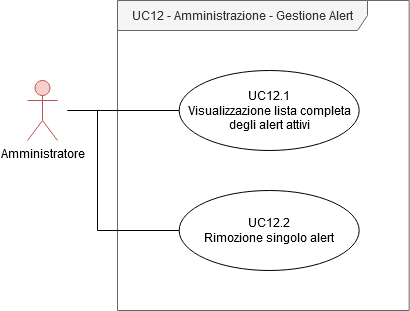
\includegraphics[scale=0.60]{res/images/uc12}
			\caption{Diagramma che descrive la gestione alert a livello amministrativo.}
		\end{figure}

		\begin{itemize}
			\item \textbf{Attori Primari}: Amministratore.
			\item \textbf{Descrizione}: L'utente navigando nella gestione degli \glock{alert} impostati dagli enti all'interno del sistema.
			\item \textbf{Precondizione}: L'utente è autenticato nella web app.
			\item \textbf{Postcondizione}: L'utente ha visualizzato o gestito gli \glock{alert} all'interno del sistema.
			\item \textbf{Scenario Principale}:
			\begin{enumerate}
				\item{L'utente, navigando nella gestione \glock{alert}, ha visualizzato o gestito gli \glock{alert} impostati dagli enti all'interno del sistema}
			\end{enumerate}	
		\end{itemize}

		\subsubsection{UC 12.1 - Visualizzazione lista completa degli alert attivi}
		\begin{itemize}
			\item \textbf{Attori Primari}: Amministratore.
			\item \textbf{Descrizione}: L'utente vuole visualizzare la lista degli \glock{alert} per tutti gli enti attivi nel sistema.
			\item \textbf{Precondizione}: L'utente sta navigando all'interno della gestione \glock{alert}.
			\item \textbf{Postcondizione}: L'utente sta visualizzando gli \glock{alert} presenti nel sistema.
			\item \textbf{Scenario Principale}:
			\begin{enumerate}
				\item{L'utente visualizza la lista degli \glock{alert} attivi nel sistema.}
			\end{enumerate}	
		\end{itemize}

		\subsubsection{UC 12.2 - Rimozione singolo alert}
		\begin{itemize}
			\item \textbf{Attori Primari}: Amministratore.
			\item \textbf{Descrizione}: L'utente vuole rimuovere un qualsiasi \glock{alert} dalla lista degli \glock{alert} attivi.
			\item \textbf{Precondizione}: L'utente sta navigando all'interno della gestione \glock{alert} e visualizza almeno un \glock{alert}
			\item \textbf{Postcondizione}: L'utente ha rimosso dal sistema l'\glock{alert} selezionato.
			\item \textbf{Scenario Principale}:
			\begin{enumerate}
				\item{L'utente seleziona un \glock{alert} dalla lista degli \glock{alert} e lo rimuove;}
				\item{L'utente non visualizza più l'\glock{alert} precedentemente selezionato.}
			\end{enumerate}	
		\end{itemize}